\documentclass[12pt]{article}
\setcounter{secnumdepth}{0} % Remove numbering
\usepackage[a4paper, left=0.9in, right=0.9in, top=1.0in, bottom=1.0in]{geometry}
\usepackage{graphicx}       % Required for inserting images
\usepackage{tocloft}        % Include the tocloft package for customizing the TOC
\usepackage{titlesec}
\usepackage{caption}
\usepackage{float}
\usepackage[newfloat]{minted}
\usepackage{stackengine}[2013-10-15]
\usepackage{color}
\usepackage{listings}
\usepackage{listings}
\usepackage{xcolor}
\definecolor{dkgreen}{rgb}{0,0.6,0}
\definecolor{gray}{rgb}{0.5,0.5,0.5}
\definecolor{mauve}{rgb}{0.58,0,0.82}

\lstset{
  language=C,
  basicstyle={\small\ttfamily},
  belowskip=3mm,
  breakatwhitespace=true,
  breaklines=true,
  classoffset=0,
  columns=flexible,
  commentstyle=\color{dkgreen},
  frame=none,
  keywordstyle=\color{blue},
  numbers=left,
  numberstyle=\tiny\color{gray},
  showstringspaces=false,
  stringstyle=\color{violet},
  tabsize=3,
  xleftmargin=1em
}

\newcommand\textss[1]{\stackengine{.9ex}{}{\scriptsize#1}{O}{l}{F}{F}{L}}

% Add a line after each section
\titleformat{\section}
  {\normalfont\Large\bfseries\centering}{\thesection}{1em}{}[{\titlerule[0.1pt]}]

\renewcommand{\cftpartleader}{\cftdotfill{\cftdotsep}}      % Adds dots between part entries
\renewcommand{\cftpartfont}{\bfseries}                      % Part entries in bold
\renewcommand{\cftpartpagefont}{\normalfont}                % Page numbers in normal font

\renewcommand{\cftsecleader}{\cftdotfill{\cftdotsep}}       % Adds dots between section entries
\renewcommand{\cftsecfont}{\bfseries}                       % Section entries in bold
\renewcommand{\cftsecpagefont}{\normalfont}                 % Page numbers in normal font

\renewcommand{\cftsubsecleader}{\cftdotfill{\cftdotsep}}    % Adds dots between subsection entries
\renewcommand{\cftsubsecpagefont}{\normalfont}              % Page numbers in normal font

\setlength{\cftbeforepartskip}{0.5em}                       % Adjust the space before part entries
\setlength{\cftbeforesecskip}{0.3em}                        % Adjust the space before section entries
\setlength{\cftbeforesubsecskip}{0.1em}                     % Adjust the space before subsection entries

\renewcommand*\contentsname{}

\begin{document}

\thispagestyle{empty}   % Removes page number from the first page
\begin{center}
    \vspace*{\fill}     % Vertically center content

    \huge Colegiul National Bilingv

    \huge "George Cosbuc"

    \vspace{4cm}

    \textbf{\Huge The Impact of C, UNIX, and Pioneers Dennis Ritchie \& Ken Thompson}

    \vspace{10cm}

    \begin{minipage}[t]{0.5\textwidth}
        \Large \textbf{Elev:}
        \large Sorin-Andrei Tudose \\
        \Large \textbf{Clasa:}
        \Large $12R_2$
    \end{minipage}%
    \begin{minipage}[t]{0.5\textwidth}
        \raggedleft
        \Large \textbf{Profesor indrumator:} \\
        \large Kerestély Melinda Laura
    \end{minipage}

    \vspace*{\fill}     % Vertically center content
\end{center}

\newpage
\begin{center}
    \vspace*{\fill}     % Vertically center content
    \Huge\textbf{Table of Contents}
    \par\noindent\rule{\textwidth}{0.4pt}
    \small\tableofcontents
    \vspace*{\fill}     % Vertically center content
\end{center}

\newpage
\section{Synopsis}
What has always fascinated me is computer programming and software engineering. After a few years of using a computer as a means of playing games, I started wondering how those applications run and what their build process is like. There were a few questions to which I really needed answers, such as: How are games and other applications built?, How are different pieces of information displayed on the screen?, How can one master the necessary skills to write a computer program?, etc. So I started doing research. Even though at that time the documentation I was reading overwhelmed me, I managed to understand that if one had the necessary knowledge, the possibilities in software engineering were endless. Since I wrote my first "Hello world" in C\texttt{++}, when I was 15 years old, I have known that hardware and software were the area I wanted to excel in. I find it truly magical how people can manipulate every pixel of a computer screen and display any desired content.\newline\newline
As a result, creating code and building applications that help solve different problems and enable us to be more effective is what I am keen on pursuing in the near future. It is, undoubtedly, a complex field where mathematical and physics skills are required, but the excitement and passion for this field help me overcome all challenges. \newline\newline
Having said that, I decided to write my Grade 12 Graduation Paper on Dennis Ritchie and Ken Thompson, who in 1969 at Bell Telephone Laboratories revolutionized  the way people used computers. Not only did they create the UNIX operating system which is the root of many modern operating systems, but they also developed the C programming language. I, for one, am amazed by the things they created considering the fact that resources were not as broadly available as they are nowadays. There were almost no applications designed for creating software and no internet that could assist with the process. In addition, they also had to write most of the code in Machine Language, a low level programming language which takes a long time to master.
\begin{center}
    Throughout this thesis we will go on a journey tracing the origins of computers.
\end{center}

\newpage

\section{Introduction}
These days, most people own at least one modern computer for personal usage. However, many do not know that the original design looked nothing like it does today.\newline\newline
First and foremost, there were no operating systems, programming languages, mice or key- boards. Moreover, there was no physical storage (solid-state drives or hard disk drives), RAM memory (random access memory) or ROM memory (read only memory). ENIAC (Electronic Numerical Integrator and Computer), the very first computer designed at the University of Pennsylvania in 1945 to serve as a military tool to properly calculate the angle of elevation of a gun. This computer consumed around 150,000 watts, which is significantly higher than modern computers (200-500 watts).\newline\newline \textbf{So how did ENIAC work?}\newline\newline
Not only did it use several cables and switches, which were used to start, shut down and control the flow of data, but also plugboards, electrical switchboards into which electrical plugs were inserted to create different temporary circuits for transmitting instructions to the machine. As a result, for each task the computer needed manual calibration which meant rewiring the plugboards and adjusting the switches. This “programming” method was not efficient in terms of flexibility and speed.

\begin{center}
    \footnotesize\textit{“Preparing ENIAC for a series of runs was an incredibly involved process. 
    First, detailed instructions had to be written defining the problem and a procedure for solving it. 
    These instructions were programmed by adjusting switches manually and inserting thousands of cables into as many as forty large plug boards. 
    A team of five operators might work several days on the external wiring and many more days searching for errors and correcting them.”}
    — Breakthrough to the Computer Age, Harry Wulforst, Charles Scribner’s \& Sons Pub., 1982
\end{center}

\noindent After experimenting with ENIAC, people found different ways to make significant improvements:
\begin{itemize}
    \item (1949) \textbf{EDSAC} and \textbf{EDVAC} - Computers get memory as tubes with mercury
    \item (1949) \textbf{BINAC} - Programming languages were introduced (William Schmitt – Short Order Code)
    \item (1952) \textbf{IBM 701} - The first computer to use the assembler-style language (low-level programming language, used to directly communicate with the computer hardware) and a repository to store frequently used blocks of data.\newline
\end{itemize}

\newpage

\section{Chapter 1: Dennis Ritchie \& Ken Thompson: C \& UNIX Pioneers}
During the late 1960s and early 1970s, Ken Thompson and Dennis Ritchie worked as colleagues at the Bell Telephone Laboratories. Brian Kerninghan, who was part of the technical staff at Bell Labs, describes Dennis Ritchie as \textit{”a really nice guy”}, who was really smart. Moreover, Kerninghan also acknowledges that Ritchie and Thompson had almost the same thinking process when creating computer algorithms. They met around 1968, when Belle Labs was famous for its research of transistors and other small research projects. Ritchie and Thompson were told to: \textit{”investigate interesting problems in computer science”}.
\newline\newline
They decided to create an operating system that  supported  multitasking,  allowing users to run programs simultaneously. The operating system was mostly done by Thompson, but Ritchie had a great contribution during the development of the filing system.\newline\newline
Working together, they developed the UNIX Operating System using the high-level C programming language designed by Ritchie. The main issue this operating system solved was the compatibility between machines. T Computer software was specific to the hardware, therefore users would come to find themselves using a machine with completely new command and operating procedures.  UNIX, being written using the C programming language, made it portable and adaptable. Moreover, UNIX also introduced pipes, which I briefly described in the introduction section. This allowed different processes to communicate with each other and thus created the possibility to run more complex tasks, more powerful workflows and automation. \newline\newline
One true passion that Ken Thompson had was computer games. In a video from the National Inventor’s Hall of Fame, Thompson says: \textit{"Unix was built for me. I didn't build it as an operating system for other people, I built it to do games and do my stuff."}. Before the ending of the video, the narrator states: \textit{"Sometimes inventions come from an individual's pursuit to push the limits of existing technology for their own use. Often this pursuit ends up benefiting us all."}.\newline\newline
Taking into consideration the limitation of computer hardware and software at that time, game development was quite the challenge for software engineers. Therefore, it took a lot of creativity and technical skills to successfully create a game. Not only did this hobby help him develop his algorithmic thinking, but it also gave Thompson a deeper understanding of early computer systems.\newline\newline
Similarly, in high school, in the 11\textss{th} grade I had the chance to participate in a Game Jam, together with four other classmates. Having only two days to complete our game required us to work as efficiently as possible by dividing the workload. There was a lot of research to conduct, since all of us had nearly no experience in game development. As a result, at the end of the contest I found myself grateful for taking up this challenge as it helped me develop a completely new skill. After all our efforts, our game won the event and we won the prize: a trip to Berlin. Little did we know that this would not be a casual trip. We took part in two extraordinary events: firstly, we were taken to a game development center, where a couple of pro programmers introduced us to different types of software used in the industry.  Moreover,  they also took a look at our game,  giving us remarkable feedback on how to improve our work. After returning home, I realised how eye-opening this whole experience had been. I found my deep passion in both software engineering and mathematics and started to work slowly on these skills, trying to learn something new every day.\newline\newline
In \textbf{1983}, Dennis Ritchie and Ken Thompson were given the Turing Award from the ACM (Association for Computing Machinery) and the citation on the reward was:
\begin{center}
    \footnotesize \textit{"The success of the Unix system stems from its tasteful selection of a few key ideas and their elegant implementation. The model of the Unix system has led a generation of software designers to new ways of thinking about programming. The genius of the Unix system is its framework, which enables programmers to stand on the work of others"}
\end{center}
In \textbf{1990} they received the IEEE Hamming Medal \textit{”for the origination of the UNIX operating system and the C programming language”}.\newline\newline
In \textbf{1998}, President Bill Clinton awarded them the National Medal of Technology \textit{"for co-inventing the UNIX operating system and the C programming language which together have led to enormous advances in computer hardware, software, and networking systems and stimulated growth of an entire industry, thereby enhancing American leadership in the Information Age"}.\newline\newline
Last but not least, in \textbf{2011} they received the Japan Prize for developing \textit{"the UNIX operating system which has significantly advanced computer software, hardware and networks over the past four decades, and facilitated the realization of the Internet."}\newline\newline
Ritchie and Thompson were able to forge paths into uncharted territory, enabling young minds to create and contribute to the world of computers. Having said that, they undoubtedly left their mark on the world, by creating a revolutionary, accessible and easy to use operating system alongside a programming language that is widely used to this day.

\newpage

\section{Chapter 2: UNIX, the operating system revolution}

The UNIX Operating System was one of the first to be written in the C programming lan- guage (initially it was written in assembly language, but later in 1972 it was rewritten), which was a big step in shifting developers to write programs efficiently using a more user friendly language without losing the ability to interact directly with the hardware. Not only did this OS put forward new features such as the hierarchical file system and the command line interface, but it also created the idea of a computer process and files. The operating system was formally presented for the first time in 1973. After the announcement, many users and companies wanted to buy the software, but unfortunately Bells Labs was forbidden to enter any business. Despite all restrictions, Ken Thompson discreetly started to answer requests, by sending tapes and disks, containing the software. All packages were accompanied with the message: ’Love, Ken’. It was in 1973 that AT\&T released Version 5 Unix which was used for educational purposes. In 1976, Version 6 was licensed for companies to use. Commercial usage was rarely seen since one licence was about \$20,000 USD (\$113,247 USD in 2023).\newline\newline
The UNIX architecture consists in 3 key parts: the kernel, the shell, and user commands. It contains several other secondary components which together provide portability, stability and interoperability across a wide range of devices. UNIX is a modular operating system (one that is built using independent components where adding or removing one does not affect the system as a whole). The Kernel is the key program that controls most of the computer resources and it is responsible for allowing processes to communicate with one another. The way users interact with UNIX based systems is quite simple. One can write a command in the shell, a CLI (command line interface) that is ultimately passed to the Kernel which initiates the correct system utility. For example, a user might use the \textit{\textbf{ls}} command. When this prompt is executed, the kernel runs the program associated to \textit{\textbf{ls}} which lists all the files in the current directory.\newline\newline
Although at that time UNIX was a revolutionary scientific invention, nowadays UNIX based operating systems have no more than 5.5\% market share. Nevertheless, operating systems such as Mac OS or Android use UNIX as a framework (a structure that you can use to build software on). For example, Android systems use the Linux Kernel (Linux is a modular Unix-like operating system, deriving much of its basic design from principles established in Unix). I have been using a UNIX like operating system for two years now. From a developer point of view, I must say it is much more convenient to write code in Linux. Not only is third party software easily accessible, but the OS is also customizable, enabling the user to create an environment which contains only the necessary software. On the other hand, different applications can have compatibility issues or sometimes might not even be available on Linux. This is because this OS withholds only 3.88\% of the market share and therefore it is not always targeted by developers when creating new software. However, over the last few years this has improved a lot, all basic applications which are found on more popular operating systems such as Windows or Mac OS being available. Moreover, Linux 
is appreciated for its native support for programming tools and libraries. All in all, despite the fact that at first there were many functionalities I did not know how to use let alone be aware of their existence , I consider Linux to be an open-source (anyone can see, modify, and distribute the code as they see fit), versatile, reliable and secure software with a great development environment.

\newpage

\section{Chapter 3: The C programming language}

This chapter will not only present the architecture of the C programming language by showcasing basic functionalities and examples, but it will also dive into the type of industries it is used in.\newline\newline
The C programming language is a GPL (general-purpose programming language used in a wide variety of application domains) created by Dennis Ritchie in 1970 to build utilities used in UNIX. Although its usage in application software has gone down, it is demanded in operating systems, device drivers (a driver is a piece of software which helps hardware communicate with the operating system), micro controllers and embedded systems (computer hardware and software designed for a specific task, for example a washing machine).\newline\newline The design of the C programming language was made in a way that could provide the user with low-level access to memory. It is a procedural language which needs to be compiled (the human readable code is transformed into machine code, 0s and 1s). The compiler itself is a program. As a side note, the steps a program goes through in order to become an executable file are the following: preprocessing, compiling, assembling and linking. Only after all these steps is the executable -the final version of the program everyone is familiar with and has on their desktops- created. For example, lets take a look at the following C program, which simply prints the string ”Hello, world!” to the console screen:
\begin{center}
    \begin{lstlisting}[language=C]
    #include <stdio.h>
    
    int main(void)
    {
        printf("Hello World!");
        return 0;
    }
    \end{lstlisting}
\end{center}

\begin{enumerate}
    \item \underline{Preprocessing} - The preprocessor directive \textbf{$\#include <stdio.h>$} instructs the compiler to add the \textbf{stdio.h} library. This is a file where the definition of the \textbf{printf} function is located. To put it in simpler terms, the compiler searches for the file called \textbf{stdio.h} on the computer and it adds its contents to the file you wrote the initial code in. 
    
    \item \underline{Compiling} - The preprocessed code is transformed in assembly language specific to the targeted user platform

    \item \underline{Assmebling} - The assembly code is translated into binary code using a computer program called "assembler"

    \item \underline{Linking} - It combines all the binary data with any other libraries. In our case, the binary code for the \textbf{printf} function will be added to our executable file.
\end{enumerate}
The syntax is free-form, which means that the position of the characters matters. For example, semicolons terminate statements and curly braces are used to group statements. In addition it consists in a fixed number of keywords such as:

\begin{enumerate}
    \item \textbf{if/else} conditional statement - This evaluates a condition and checks weather it is true or false
    \begin{lstlisting}[language=C]
        If (Boolean condition) Then
           (consequent)
        Else
           (alternative)
        End If
    \end{lstlisting}

    \item \textbf{for} loops - This is called a control flow statement. It runs a group of instructions until a certain condition is met. The following example calls the function \textbf{test()} until the variable \textbf{i} reaches \textbf{99}, doing a total of \textbf{100} iterations.
    \begin{lstlisting}[language=C]
        for (i = 0; i < 100; i++) {
            test();
        }
    \end{lstlisting}

    \item \textbf{while} loops - A control flow statement which executes a block of code until a boolean condition is met. In the example listed above we will replace the \textbf{for} loop with a \textbf{while} loop. Thus we will need to add another instruction inside the loop which adds \textbf{1} to the variable \textbf{i}. Moreover, \textbf{i} needs to be given the value \textbf{0} before entering the loop.
    \begin{lstlisting}[language=C]
        i = 0;
        while (i < 100)
        {
            test();
            i++;
        }
    \end{lstlisting}

    \item \textbf{do-while} loops - A control flow statement which executes a block of code until a boolean condition is met. It is known as a \textbf{\underline{post-test}} loop since the only difference between a \textbf{while} loop and a \textbf{do-while} loop is which moment of the execution the boolean condition is validated. What needs to be noted is that if \textbf{do-while} were used in the example above an extra iteration would take place. Therefore, in the new example below, I added an additional conditional statement that checks weather \textbf{i} is greater or equal to \textbf{100}. If \textbf{i} reached \textbf{100} the \textbf{break} keyword is used in order to exit the loop.
    \begin{lstlisting}[language=C]
        i = 0;
        do
        {   
            if (i + 1 >= 100)
                break;
            i++;
            test();
        } while (i < 100);
    \end{lstlisting}
\end{enumerate}
Arithmetic, bitwise (operation at the level of each individual bit) and logic operators are also supported: +, +=, ++, \&, $||$, etc. Having said that, there are many other features provided by the C programming language such as: heterogeneous aggregate data types (\textbf{struct} - allows custom variable types to be created which are made out of other data types), \textbf{union} (it allows multiple data types to share the same memory location), \textbf{array} (there is no \textit{"array"} keyword; however the concept is indicated by square brackets, for example \textbf{v[10]}), \textbf{enum} and \textbf{string}, which is implemented using a character array.\newline\newline
Other key features which need to be noted are:

\begin{enumerate}
    \item Procedures (a type \textbf{void} - 'empty' function which does not return a value, only performs instructions). 

    \begin{lstlisting}[language=C]
        void factorial(unsigned int n);
        void sum(int x, int y);
        void concat(char *name, char *surname);
    \end{lstlisting}

    \item Low level access to computer memory using pointers (an object which stores a memory address). Keep in mind that the pointer itself has a memory address which can also be stored. For example, let us declare a variable which can store a natural number and assign it the number \textbf{10}:

    \begin{lstlisting}[language=C]
        unsigned int n = 10;
    \end{lstlisting}

    This variable is mapped in the computer address at a specific address: \textbf{0x7ffe56ffd18c}. Now we can use a special variable called a pointer to store the address associated to \textbf{n}.

    \begin{lstlisting}[language=C]
        unsigned int n = 10, *p;
        p = &n;
    \end{lstlisting}

   Using the ”$\&$” (Address-of Operator) we retrieve the address of the variable n and we assign it to our pointer \textbf{p}. The following example presents some operations that can be done using pointers:

    \begin{lstlisting}[language=C]
        #include <stdio.h>

        int main() 
        {
            unsigned int n = 10, *p;
            p = &n;
        
            printf("Value of n: %u\n", n);
            printf("Address stored in p: %p\n", p);
        
            *p = 20;
            printf("Updated value of n: %u\n", n);
        
            *p += 5;
            printf("Value of n after increment: %u\n", n);
        
            return 0;
        }
    \end{lstlisting}

    \textbf{Console output:}
    \begin{lstlisting}[language=C]
        Value of n: 10
        Address stored in p: 0x7ffe56ffd18c
        Updated value of n: 20
        Value of n after increment: 25
    \end{lstlisting}
    
    \item Recursion - The ability of a function to call itself. In the example below, we want to calculate \textbf{n!} (5! = 1 * 2 * 3 * 4 * 5 = 120) using recursion. Firstly, the base case needs to be set. This is where the function will stop calling itself. In this case, when n reaches 0 or 1 the program should return 1 (1! = 1 and 0! = 1). When the base case is reached each return value is traced back and multiplied with the previous value until we reach back to the first function call.
    \begin{itemize}
        \item Initial Call: factorial(5) is called.
        \item Recursive Call 1: Inside factorial(5), since n is not 0 or 1, it calculates 5 * factorial(4).
        \item Recursive Call 2: Inside factorial(4), it calculates 4 * factorial(3).
        \item Recursive Call 3: Inside factorial(3), it calculates 3 * factorial(2).
        \item Recursive Call 4: Inside factorial(2), it calculates 2 * factorial(1).
        \item Base Case Reached: Inside factorial(1), the base case is met (n == 1), so it returns 1.
    \end{itemize}
    
    \begin{lstlisting}[language=C]
        int factorial(int n) 
        {
            // Base case
            if (n == 0 || n == 1) 
                return 1;
            else
                // Recursive case: n! = n * (n-1)!
                return n * factorial(n - 1); 
        }
    \end{lstlisting}

    \item \textbf{static/extern} attributes which control where a function/variable is visible in other files. Let's take a look at the following examples:
    \begin{itemize}
        \item Static local variables \newline
        When the function \textbf{add()} is called the first time, it declares the static variable number which stores the number \textbf{10}. Immediately after that, it adds 1 and returns the value (11) which will be printed to the console screen. However, contrary to popular belief when the second call of the function is initiated, the variable ”number” will not be reassigned, but it will still be \textbf{11}. Therefore the second \textbf{printf} will print the number \textbf{12} on the screen. \newpage
        \begin{lstlisting}[language=C]
        #include <stdio.h>
        
        int add(void) 
        {
            static int number = 10;
            number++;
            return number;
        }
        
        int main(void) 
        {
            printf("%d\n", add()); /* Prints 11 */
            printf("%d\n", add()); /* Prints 12 */
            return 0;
        }
        \end{lstlisting}

        \item Static Function - Not only is a \textbf{non-static} function visible throughout the program (globally), but it can also be called outside the file where it was created. The static attribute limits the function scope, to be called only inside the file where it was declared and defined.
        \begin{lstlisting}[language=C]
        static void function(void)  
        {  
            printf("Hello World!");  
        }  
        \end{lstlisting}

        \item Static Global Variable - Similar to a static function, the global property is kept, but its scope is limited to the file it was declared in.
        \begin{lstlisting}[language=C]
        static unsigned int glob_var;
        \end{lstlisting}

        \item Extern Variable - This keyword announces the existence of the variable to the compiler, however it does not allocate any memory to it. For example, let's create the files main.c, helper.c and helper.h (a header file contains function or variable definitions, macros, etc, which we import using \textbf{\#include "file\_name"}).
        \begin{itemize}
            \item main.c
            \begin{lstlisting}[language=C]
            #include <stdio.h>
            #include "helper.h"
            
            int main() 
            {
                printf("%d\n", ext_var);
            
                print(20);
            
                return 0;
            }
            \end{lstlisting} \newpage

            \item helper.c
            \begin{lstlisting}[language=C]
            #include <stdio.h>
            #include "helper.h"
            
            unsigned int ext_var = 10;
            
            void print(unsigned int x)
            {
                printf("%u\n", x);
            }
            \end{lstlisting}

            \item helper.h
            \begin{lstlisting}[language=C]
            #ifndef HELPER_H_
            #define HELPER_H_
            
            extern unsigned int ext_var;
            
            extern void print(unsigned int x);
            
            #endif
            \end{lstlisting}
        \end{itemize}
    \end{itemize}
\end{enumerate}
In the file \textbf{main.c} the program tries to print the value of the variable called \textbf{ext\_var}. It finds the declaration inside the header file, but the extern keyword tells the compiler ”look outside my scope and you will find the definition”, which is located in \textbf{helper.c}. The same concept applies to extern functions.\newline\newline
C was the foundation of many other languages such as: C\texttt{++}, C\texttt{\#}, UNIX’s C shell, D, Go, Java, JavaScript, Julia, Limbo, LPC, Objective-C, Perl, PHP, Python, Ruby, Rust, Swift, Verilog and System Verilog (hardware description languages). With this in mind, in 1979, a Danish computer scientist Bjarne Stroustrup developed the C\texttt{++} programming language at Bell Labs. It was created as an extension of C, which also included high-level features for program organisation such as: OOP (object oriented programming), templates, STL (Standard Template Library), etc. The creator describes the language as \textit{”a light-weight abstraction programming language [designed] for building and using efficient and elegant abstractions”} and \textit{”offering both hardware access and abstraction is the basis of C++. Doing it efficiently is what distinguishes it from other languages.”}. 

\newpage
\section{Conclusion}
This paper puts into perspective the origins of computers, while presenting the evolution of our means of communicating with hardware through programming languages. We started off by going back to 1945 when the first computer was created (ENIAC) and made our way to 1979 when \texttt{C++} was invented. Moreover, I felt the need to include different examples in order to better understand the functionalities and mechanisms of the C programming language. Therefore, I wrote several fairly easy computer programs which help readers correlate the explanations with the syntax. \newline\newline To my mind, C is the backbone of today’s modern computer systems and I do not believe that this will change very soon. It is nonetheless a fast and efficient language which is worth learning, as it beats most modern programming languages like Python or Go, in terms of speed. I highly recommend getting familiar with these low level programming languages (C/C\texttt{++}), since it gives developers a better understanding of what is actually going on under the hood. \newline\newline All in all, with the help of this thesis not only was I able to present the legendary Ken Thomson and Dennis Ritchie, who left an incredible mark on computer engineering as a whole, but I also had the chance to present my opinon on various topics related to this field.

\newpage

\vspace*{\fill}
\section{Bibliography}

\begin{enumerate}
    \item \textbf{\underline{YouTube Videos}}
    
    \begin{sloppypar}
        \footnotesize
        www.youtube.com/watch?v=g3jOJfrOknA\&ab\_channel=NationalInventorsHallofFame-NIHF \\
        https://www.youtube.com/watch?v=JoVQTPbD6UY\&ab\_channel=VortexTech \\
        https://www.youtube.com/watch?v=umF6SNYaJNw\&ab\_channel=Alsarhan \\
        https://www.youtube.com/watch?v=EY6q5dv\_B-o\&ab\_channel=VintageComputerFederation \\
        https://bigthink.com/videos/why-i-created-c/
    \end{sloppypar}

    \item \textbf{\underline{Websites}}
    \begin{sloppypar}
        \footnotesize
        https://dsf.berkeley.edu/cs262/unix.pdf \\
        https://www.ibm.com/docs/en/cics-ts/5.3?topic=applications-example-assembler-language-program-leasm \\
        https://people.cs.rutgers.edu/~pxk/416/notes/01-intro.html
    \end{sloppypar}

    \item \textbf{\underline{Books}}
    \begin{sloppypar}
        \footnotesize
        Breakthrough to the Computer Age, Harry Wulforst, Charles Scribner’s \& Sons Pub., 1982
    \end{sloppypar}
\end{enumerate}

\vspace*{\fill}

\newpage
\section{Appendix}

\begin{itemize}
    \item ENIAC - The first computer (1945)
    \begin{figure}[H]
        \centering
        \captionsetup{labelformat=empty}
        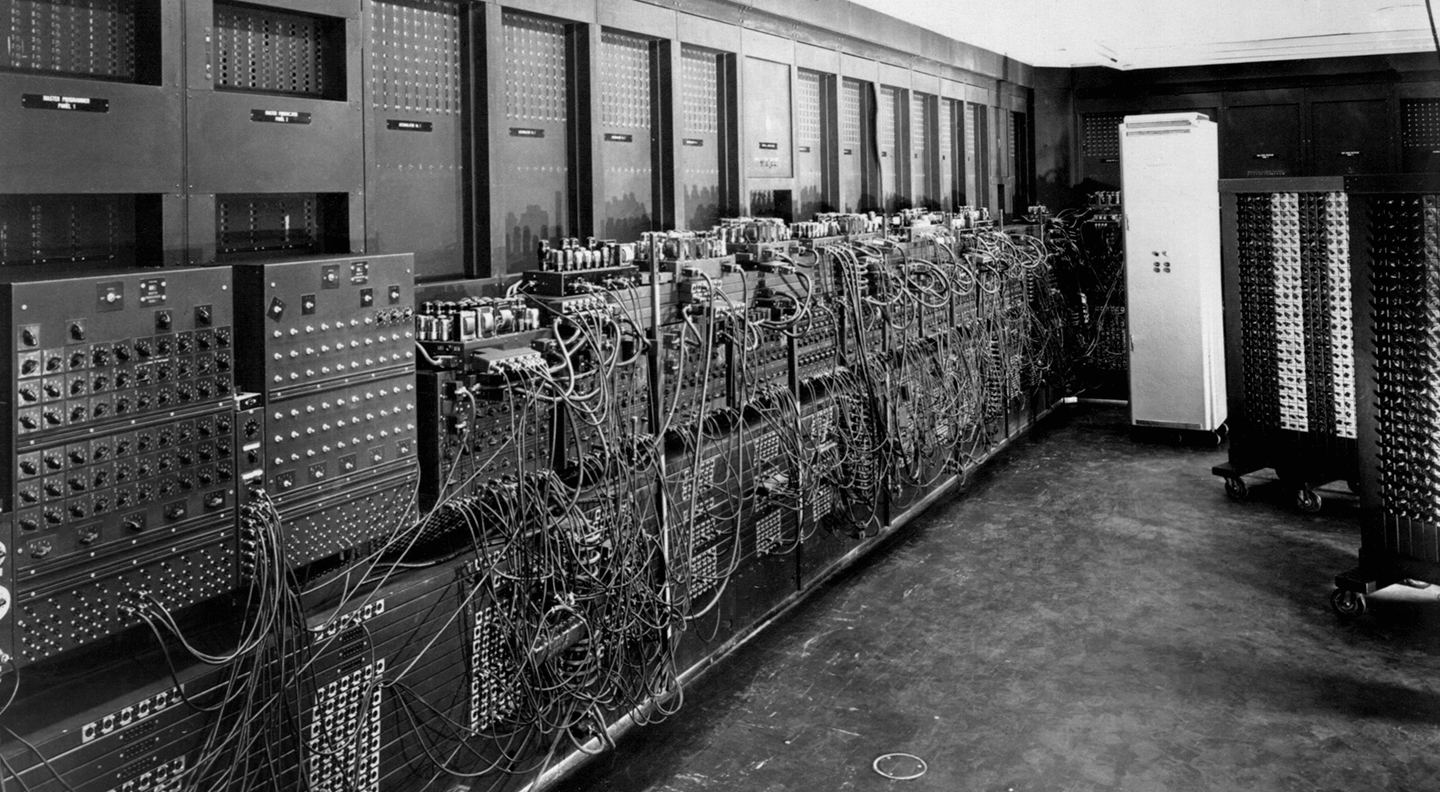
\includegraphics[width=420px]{images/ENIAC.png}
        \label{fig:enter-label}
    \end{figure}

    \item Ken-Thomson and Dennis Ritchie developing UNIX (late 1960s and early 1970s)
    \begin{figure}[H]
        \centering
        \captionsetup{labelformat=empty}
        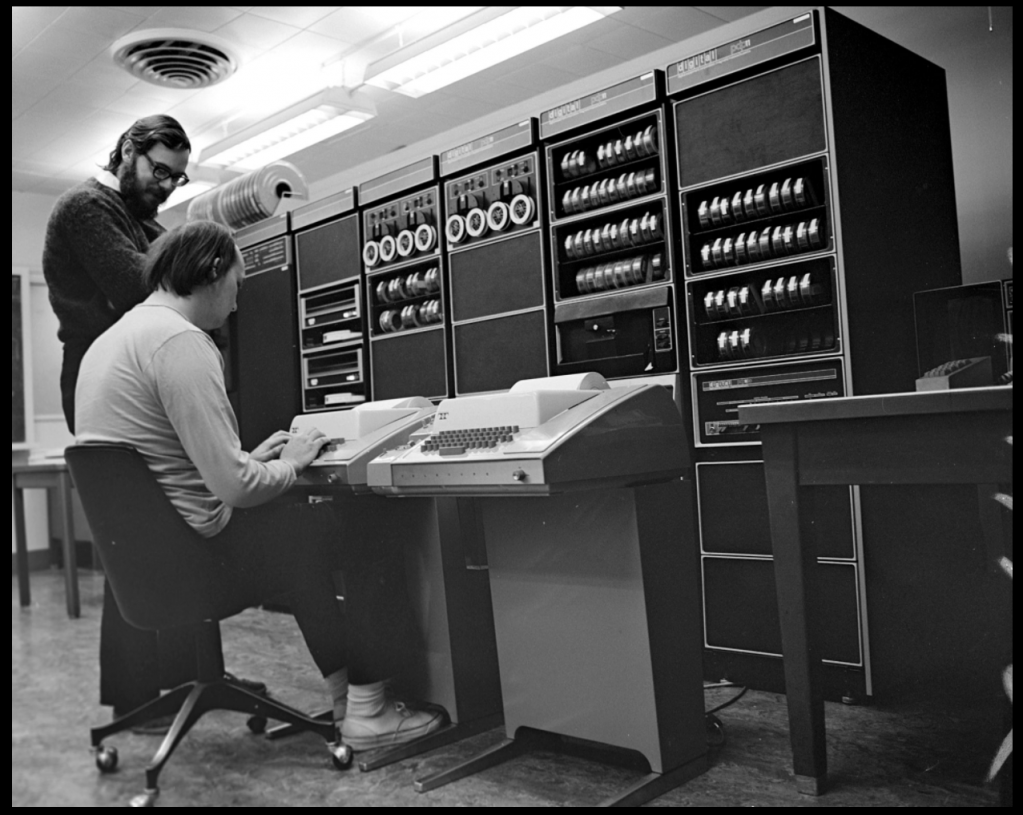
\includegraphics[width=420px]{images/Ken_Dennis.png}
        \label{fig:enter-label}
    \end{figure}

    \item Thmopson (left) and Ritchie (center) receiving the National Medal of Technology from president Clinton in 1999
    \begin{figure}[H]
        \centering
        \captionsetup{labelformat=empty}
        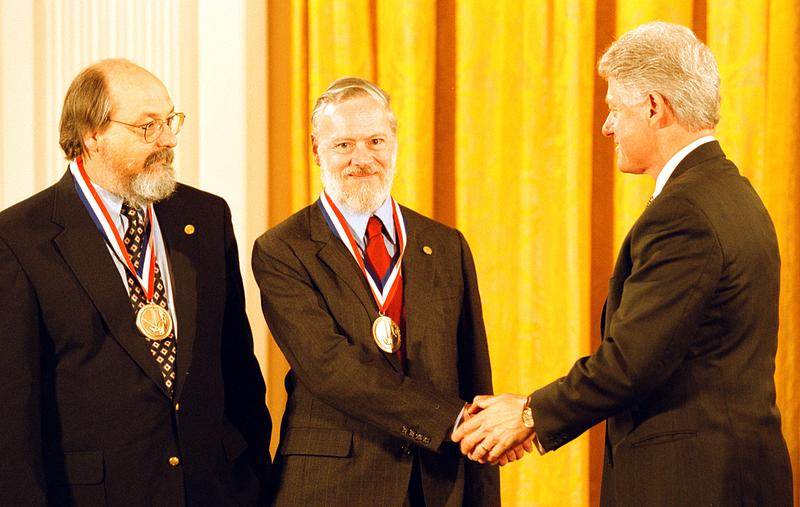
\includegraphics[width=420px]{images/Ken-Thompson-Dennis-Ritchie-and-Bill-Clinton.jpg}
        \label{fig:enter-label}
    \end{figure}

    \item Bell Labs Holmdel Complex - Holmdel Township, New Jersey, U.S.
    \begin{figure}[H]
        \centering
        \captionsetup{labelformat=empty}
        \includegraphics[width=420px]{images/Bell_Labs_Holmdel.jpg}
        \label{fig:enter-label}
    \end{figure}
\end{itemize}

\end{document}